% Options for packages loaded elsewhere
\PassOptionsToPackage{unicode}{hyperref}
\PassOptionsToPackage{hyphens}{url}
\PassOptionsToPackage{dvipsnames,svgnames,x11names}{xcolor}
%
\documentclass[
  letterpaper,
  DIV=11,
  numbers=noendperiod]{scrartcl}

\usepackage{amsmath,amssymb}
\usepackage{iftex}
\ifPDFTeX
  \usepackage[T1]{fontenc}
  \usepackage[utf8]{inputenc}
  \usepackage{textcomp} % provide euro and other symbols
\else % if luatex or xetex
  \usepackage{unicode-math}
  \defaultfontfeatures{Scale=MatchLowercase}
  \defaultfontfeatures[\rmfamily]{Ligatures=TeX,Scale=1}
\fi
\usepackage{lmodern}
\ifPDFTeX\else  
    % xetex/luatex font selection
\fi
% Use upquote if available, for straight quotes in verbatim environments
\IfFileExists{upquote.sty}{\usepackage{upquote}}{}
\IfFileExists{microtype.sty}{% use microtype if available
  \usepackage[]{microtype}
  \UseMicrotypeSet[protrusion]{basicmath} % disable protrusion for tt fonts
}{}
\makeatletter
\@ifundefined{KOMAClassName}{% if non-KOMA class
  \IfFileExists{parskip.sty}{%
    \usepackage{parskip}
  }{% else
    \setlength{\parindent}{0pt}
    \setlength{\parskip}{6pt plus 2pt minus 1pt}}
}{% if KOMA class
  \KOMAoptions{parskip=half}}
\makeatother
\usepackage{xcolor}
\setlength{\emergencystretch}{3em} % prevent overfull lines
\setcounter{secnumdepth}{5}
% Make \paragraph and \subparagraph free-standing
\makeatletter
\ifx\paragraph\undefined\else
  \let\oldparagraph\paragraph
  \renewcommand{\paragraph}{
    \@ifstar
      \xxxParagraphStar
      \xxxParagraphNoStar
  }
  \newcommand{\xxxParagraphStar}[1]{\oldparagraph*{#1}\mbox{}}
  \newcommand{\xxxParagraphNoStar}[1]{\oldparagraph{#1}\mbox{}}
\fi
\ifx\subparagraph\undefined\else
  \let\oldsubparagraph\subparagraph
  \renewcommand{\subparagraph}{
    \@ifstar
      \xxxSubParagraphStar
      \xxxSubParagraphNoStar
  }
  \newcommand{\xxxSubParagraphStar}[1]{\oldsubparagraph*{#1}\mbox{}}
  \newcommand{\xxxSubParagraphNoStar}[1]{\oldsubparagraph{#1}\mbox{}}
\fi
\makeatother

\usepackage{color}
\usepackage{fancyvrb}
\newcommand{\VerbBar}{|}
\newcommand{\VERB}{\Verb[commandchars=\\\{\}]}
\DefineVerbatimEnvironment{Highlighting}{Verbatim}{commandchars=\\\{\}}
% Add ',fontsize=\small' for more characters per line
\usepackage{framed}
\definecolor{shadecolor}{RGB}{241,243,245}
\newenvironment{Shaded}{\begin{snugshade}}{\end{snugshade}}
\newcommand{\AlertTok}[1]{\textcolor[rgb]{0.68,0.00,0.00}{#1}}
\newcommand{\AnnotationTok}[1]{\textcolor[rgb]{0.37,0.37,0.37}{#1}}
\newcommand{\AttributeTok}[1]{\textcolor[rgb]{0.40,0.45,0.13}{#1}}
\newcommand{\BaseNTok}[1]{\textcolor[rgb]{0.68,0.00,0.00}{#1}}
\newcommand{\BuiltInTok}[1]{\textcolor[rgb]{0.00,0.23,0.31}{#1}}
\newcommand{\CharTok}[1]{\textcolor[rgb]{0.13,0.47,0.30}{#1}}
\newcommand{\CommentTok}[1]{\textcolor[rgb]{0.37,0.37,0.37}{#1}}
\newcommand{\CommentVarTok}[1]{\textcolor[rgb]{0.37,0.37,0.37}{\textit{#1}}}
\newcommand{\ConstantTok}[1]{\textcolor[rgb]{0.56,0.35,0.01}{#1}}
\newcommand{\ControlFlowTok}[1]{\textcolor[rgb]{0.00,0.23,0.31}{\textbf{#1}}}
\newcommand{\DataTypeTok}[1]{\textcolor[rgb]{0.68,0.00,0.00}{#1}}
\newcommand{\DecValTok}[1]{\textcolor[rgb]{0.68,0.00,0.00}{#1}}
\newcommand{\DocumentationTok}[1]{\textcolor[rgb]{0.37,0.37,0.37}{\textit{#1}}}
\newcommand{\ErrorTok}[1]{\textcolor[rgb]{0.68,0.00,0.00}{#1}}
\newcommand{\ExtensionTok}[1]{\textcolor[rgb]{0.00,0.23,0.31}{#1}}
\newcommand{\FloatTok}[1]{\textcolor[rgb]{0.68,0.00,0.00}{#1}}
\newcommand{\FunctionTok}[1]{\textcolor[rgb]{0.28,0.35,0.67}{#1}}
\newcommand{\ImportTok}[1]{\textcolor[rgb]{0.00,0.46,0.62}{#1}}
\newcommand{\InformationTok}[1]{\textcolor[rgb]{0.37,0.37,0.37}{#1}}
\newcommand{\KeywordTok}[1]{\textcolor[rgb]{0.00,0.23,0.31}{\textbf{#1}}}
\newcommand{\NormalTok}[1]{\textcolor[rgb]{0.00,0.23,0.31}{#1}}
\newcommand{\OperatorTok}[1]{\textcolor[rgb]{0.37,0.37,0.37}{#1}}
\newcommand{\OtherTok}[1]{\textcolor[rgb]{0.00,0.23,0.31}{#1}}
\newcommand{\PreprocessorTok}[1]{\textcolor[rgb]{0.68,0.00,0.00}{#1}}
\newcommand{\RegionMarkerTok}[1]{\textcolor[rgb]{0.00,0.23,0.31}{#1}}
\newcommand{\SpecialCharTok}[1]{\textcolor[rgb]{0.37,0.37,0.37}{#1}}
\newcommand{\SpecialStringTok}[1]{\textcolor[rgb]{0.13,0.47,0.30}{#1}}
\newcommand{\StringTok}[1]{\textcolor[rgb]{0.13,0.47,0.30}{#1}}
\newcommand{\VariableTok}[1]{\textcolor[rgb]{0.07,0.07,0.07}{#1}}
\newcommand{\VerbatimStringTok}[1]{\textcolor[rgb]{0.13,0.47,0.30}{#1}}
\newcommand{\WarningTok}[1]{\textcolor[rgb]{0.37,0.37,0.37}{\textit{#1}}}

\providecommand{\tightlist}{%
  \setlength{\itemsep}{0pt}\setlength{\parskip}{0pt}}\usepackage{longtable,booktabs,array}
\usepackage{calc} % for calculating minipage widths
% Correct order of tables after \paragraph or \subparagraph
\usepackage{etoolbox}
\makeatletter
\patchcmd\longtable{\par}{\if@noskipsec\mbox{}\fi\par}{}{}
\makeatother
% Allow footnotes in longtable head/foot
\IfFileExists{footnotehyper.sty}{\usepackage{footnotehyper}}{\usepackage{footnote}}
\makesavenoteenv{longtable}
\usepackage{graphicx}
\makeatletter
\newsavebox\pandoc@box
\newcommand*\pandocbounded[1]{% scales image to fit in text height/width
  \sbox\pandoc@box{#1}%
  \Gscale@div\@tempa{\textheight}{\dimexpr\ht\pandoc@box+\dp\pandoc@box\relax}%
  \Gscale@div\@tempb{\linewidth}{\wd\pandoc@box}%
  \ifdim\@tempb\p@<\@tempa\p@\let\@tempa\@tempb\fi% select the smaller of both
  \ifdim\@tempa\p@<\p@\scalebox{\@tempa}{\usebox\pandoc@box}%
  \else\usebox{\pandoc@box}%
  \fi%
}
% Set default figure placement to htbp
\def\fps@figure{htbp}
\makeatother

\KOMAoption{captions}{tableheading}
\makeatletter
\@ifpackageloaded{caption}{}{\usepackage{caption}}
\AtBeginDocument{%
\ifdefined\contentsname
  \renewcommand*\contentsname{Table of contents}
\else
  \newcommand\contentsname{Table of contents}
\fi
\ifdefined\listfigurename
  \renewcommand*\listfigurename{List of Figures}
\else
  \newcommand\listfigurename{List of Figures}
\fi
\ifdefined\listtablename
  \renewcommand*\listtablename{List of Tables}
\else
  \newcommand\listtablename{List of Tables}
\fi
\ifdefined\figurename
  \renewcommand*\figurename{Figure}
\else
  \newcommand\figurename{Figure}
\fi
\ifdefined\tablename
  \renewcommand*\tablename{Table}
\else
  \newcommand\tablename{Table}
\fi
}
\@ifpackageloaded{float}{}{\usepackage{float}}
\floatstyle{ruled}
\@ifundefined{c@chapter}{\newfloat{codelisting}{h}{lop}}{\newfloat{codelisting}{h}{lop}[chapter]}
\floatname{codelisting}{Listing}
\newcommand*\listoflistings{\listof{codelisting}{List of Listings}}
\makeatother
\makeatletter
\makeatother
\makeatletter
\@ifpackageloaded{caption}{}{\usepackage{caption}}
\@ifpackageloaded{subcaption}{}{\usepackage{subcaption}}
\makeatother

\usepackage{bookmark}

\IfFileExists{xurl.sty}{\usepackage{xurl}}{} % add URL line breaks if available
\urlstyle{same} % disable monospaced font for URLs
\hypersetup{
  pdftitle={Michigan Graph Scheme for Stata},
  colorlinks=true,
  linkcolor={blue},
  filecolor={Maroon},
  citecolor={Blue},
  urlcolor={Blue},
  pdfcreator={LaTeX via pandoc}}


\title{Michigan Graph Scheme for Stata}
\author{Andy Grogan-Kaylor}
\date{2025-02-18}

\begin{document}
\maketitle

\renewcommand*\contentsname{Table of contents}
{
\hypersetup{linkcolor=}
\setcounter{tocdepth}{3}
\tableofcontents
}

\section{Introduction}\label{introduction}

\begin{figure}[H]

{\centering 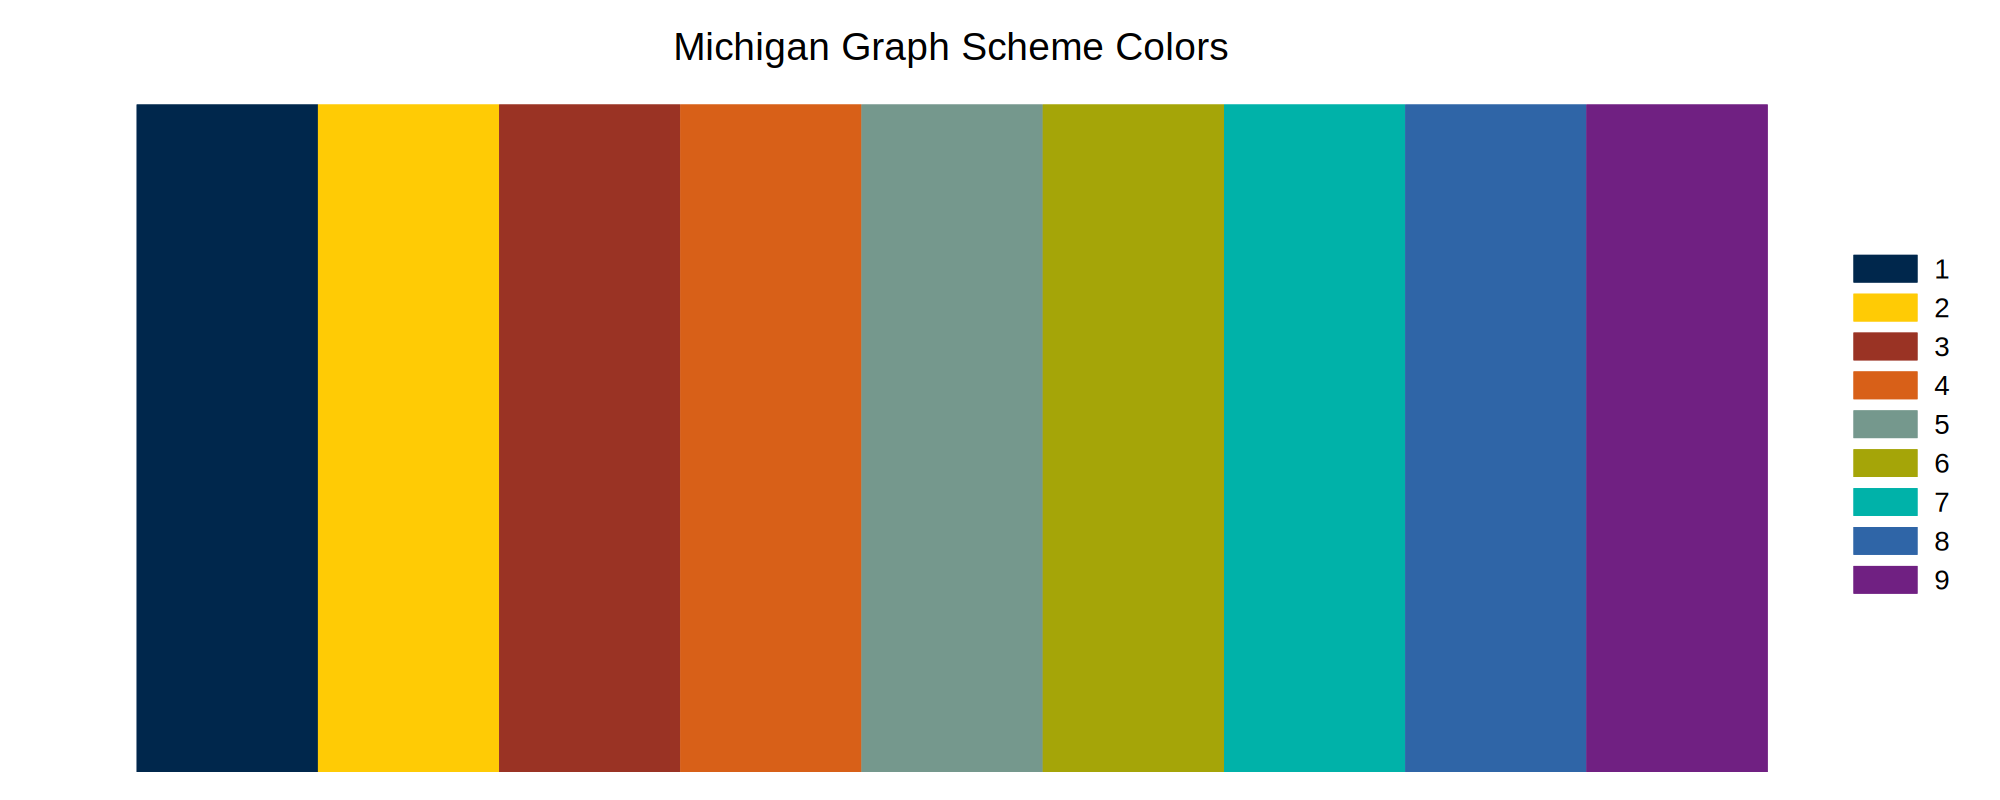
\includegraphics[width=0.75\linewidth,height=\textheight,keepaspectratio]{MichiganColorsStata.png}

}

\caption{Colors in Michigan Graph Scheme}

\end{figure}%

Stata provides the use of graph schemes that improve the overall look of
graphs.

See \texttt{help\ scheme}.

The \emph{Michigan graph scheme} makes use of official University of
Michigan colors.

\section{Installation}\label{installation}

Type \texttt{net\ from\ https://agrogan1.github.io/Stata} and click the
links to install.

\section{Example Data}\label{example-data}

We are going to use the famous ``iris'' data collected by Edgar
Anderson.

\begin{Shaded}
\begin{Highlighting}[]
\KeywordTok{clear} \OtherTok{all}
    
\KeywordTok{use} \StringTok{"iris.dta"}\NormalTok{, }\KeywordTok{clear}

\KeywordTok{summarize}
\end{Highlighting}
\end{Shaded}

\begin{verbatim}
Running /Users/agrogan/Desktop/GitHub/Stata/michigan-graph-scheme/profile.do 

> ...

    Variable |        Obs        Mean    Std. dev.       Min        Max
-------------+---------------------------------------------------------
Sepal_Length |        150    5.843333    .8280661        4.3        7.9
 Sepal_Width |        150    3.057333    .4358663          2        4.4
Petal_Length |        150       3.758    1.765298          1        6.9
 Petal_Width |        150    1.199333    .7622377         .1        2.5
     Species |        150           2    .8192319          1          3
\end{verbatim}

\section{Histogram}\label{histogram}

\begin{Shaded}
\begin{Highlighting}[]
\KeywordTok{histogram}\NormalTok{ Petal\_Length, }\DecValTok{scheme}\NormalTok{(michigan)}
\end{Highlighting}
\end{Shaded}

\begin{figure}[H]

{\centering \includegraphics[width=0.5\linewidth,height=\textheight,keepaspectratio]{myhistogram.png}

}

\caption{Histogram Using Michigan Scheme}

\end{figure}%

\section{Histogram With Transparency}\label{histogram-with-transparency}

\begin{Shaded}
\begin{Highlighting}[]
\KeywordTok{histogram}\NormalTok{ Petal\_Length, fcolor(\%50) }\DecValTok{scheme}\NormalTok{(michigan)}
\end{Highlighting}
\end{Shaded}

\begin{figure}[H]

{\centering \includegraphics[width=0.5\linewidth,height=\textheight,keepaspectratio]{myhistogram2.png}

}

\caption{Histogram Using Michigan Scheme And Slightly Transparent Bars}

\end{figure}%

\section{Bar Graph}\label{bar-graph}

\begin{Shaded}
\begin{Highlighting}[]
\KeywordTok{graph} \BaseNTok{bar}\NormalTok{ Petal\_Length, }\BaseNTok{over}\NormalTok{(Species) }\DecValTok{scheme}\NormalTok{(michigan) asyvars}
\end{Highlighting}
\end{Shaded}

\begin{figure}[H]

{\centering \includegraphics[width=0.5\linewidth,height=\textheight,keepaspectratio]{mybargraph.png}

}

\caption{Bar Graph Using Michigan Scheme}

\end{figure}%

\section{Bar Graph With Transparency}\label{bar-graph-with-transparency}

\begin{Shaded}
\begin{Highlighting}[]
\KeywordTok{graph} \BaseNTok{bar}\NormalTok{ Petal\_Length, }\BaseNTok{over}\NormalTok{(Species) intensity(70) }\DecValTok{scheme}\NormalTok{(michigan) asyvars}
\end{Highlighting}
\end{Shaded}

\begin{figure}[H]

{\centering \includegraphics[width=0.5\linewidth,height=\textheight,keepaspectratio]{mybargraph2.png}

}

\caption{Bar Graph Using Michigan Scheme and Slightly Transparent Bars}

\end{figure}%

\section{Scatterplot}\label{scatterplot}

\begin{Shaded}
\begin{Highlighting}[]
\KeywordTok{twoway}\NormalTok{ (}\KeywordTok{scatter}\NormalTok{ Petal\_Length Petal\_Width) }\CommentTok{///}
\NormalTok{(}\KeywordTok{lfit}\NormalTok{ Petal\_Length Petal\_Width), }\CommentTok{///}
\DecValTok{scheme}\NormalTok{(michigan)}
\end{Highlighting}
\end{Shaded}

\begin{figure}[H]

{\centering \includegraphics[width=0.5\linewidth,height=\textheight,keepaspectratio]{myscatter.png}

}

\caption{Scatterplot Using Michigan Scheme}

\end{figure}%

\section{Scatterplot With
Transparency}\label{scatterplot-with-transparency}

\begin{Shaded}
\begin{Highlighting}[]
\KeywordTok{twoway}\NormalTok{ (}\KeywordTok{scatter}\NormalTok{ Petal\_Length Petal\_Width, mcolor(\%30)) }\CommentTok{/// markers have 30\% transparency}
\NormalTok{(}\KeywordTok{lfit}\NormalTok{ Petal\_Length Petal\_Width), }\CommentTok{///}
\DecValTok{scheme}\NormalTok{(michigan)}
\end{Highlighting}
\end{Shaded}

\begin{figure}[H]

{\centering \includegraphics[width=0.5\linewidth,height=\textheight,keepaspectratio]{myscatter2.png}

}

\caption{Scatterplot Using Michigan Scheme And Slightly Transparent
Markers}

\end{figure}%

\section{Legend Placement}\label{legend-placement}

Sometimes you may wish to have the legend of the graph placed at the
\emph{bottom} of the graph. The \texttt{pos(6)} suboption inside the
\texttt{legend} option will place the legend at the bottom, while you
can manually control the number of legend rows with the \texttt{rows}
suboption.

\begin{Shaded}
\begin{Highlighting}[]
\KeywordTok{graph} \BaseNTok{bar}\NormalTok{ Petal\_Length, }\BaseNTok{over}\NormalTok{(Species) }\DecValTok{scheme}\NormalTok{(michigan) asyvars }\BaseNTok{legend}\NormalTok{(pos(6) }\BaseNTok{rows}\NormalTok{(1))}
\end{Highlighting}
\end{Shaded}

\begin{figure}[H]

{\centering \includegraphics[width=0.5\linewidth,height=\textheight,keepaspectratio]{mybargraph3.png}

}

\caption{Bar Graph Using Michigan Scheme and Modified Legend}

\end{figure}%

\section{Individual Michigan Colors}\label{individual-michigan-colors}

Individual University of Michigan colors are listed below.

\begin{longtable}[]{@{}
  >{\raggedright\arraybackslash}p{(\linewidth - 4\tabcolsep) * \real{0.6667}}
  >{\raggedright\arraybackslash}p{(\linewidth - 4\tabcolsep) * \real{0.1528}}
  >{\raggedright\arraybackslash}p{(\linewidth - 4\tabcolsep) * \real{0.1528}}@{}}
\toprule\noalign{}
\begin{minipage}[b]{\linewidth}\raggedright
Color
\end{minipage} & \begin{minipage}[b]{\linewidth}\raggedright
Hex
\end{minipage} & \begin{minipage}[b]{\linewidth}\raggedright
RGB
\end{minipage} \\
\midrule\noalign{}
\endhead
\bottomrule\noalign{}
\endlastfoot
\textcolor[HTML]{white}{\colorbox[HTML]{00274C}{\parbox{\linewidth}{Blue}}}
& \#00274C & 0 39 76 \\
\colorbox[HTML]{FFCB05}{\parbox{\linewidth}{Maize}} & \#FFCB05 & 255 203
5 \\
\textcolor[HTML]{white}{\colorbox[HTML]{9A3324}{\parbox{\linewidth}{Tappan
Red}}} & \#9A3324 & 154 51 36 \\
\colorbox[HTML]{D86018}{\parbox{\linewidth}{Ross School Orange}} &
\#D86018 & 216 96 24 \\
\colorbox[HTML]{A5A508}{\parbox{\linewidth}{Wave Field Green}} &
\#A5A508 & 165 165 8 \\
\colorbox[HTML]{00B2A9}{\parbox{\linewidth}{Taubman Teal}} & \#00B2A9 &
0 178 169 \\
\textcolor[HTML]{white}{\colorbox[HTML]{2F65A7}{\parbox{\linewidth}{Arboretum
Blue}}} & \#2F65A7 & 47 101 167 \\
\textcolor[HTML]{white}{\colorbox[HTML]{702082}{\parbox{\linewidth}{Ann
Arbor Amethyst}}} & \#702082 & 112 32 130 \\
\textcolor[HTML]{white}{\colorbox[HTML]{575294}{\parbox{\linewidth}{Matthaei
Violet}}} & \#575294 & 87 82 148 \\
\colorbox[HTML]{CFC096}{\parbox{\linewidth}{UMMA Tan}} & \#CFC096 & 207
192 150 \\
\colorbox[HTML]{9B9A6D}{\parbox{\linewidth}{Burton Tower Beige}} &
\#9B9A6D & 155 154 109 \\
\colorbox[HTML]{989C97}{\parbox{\linewidth}{Angell Hall Ash}} & \#989C97
& 152 156 151 \\
\textcolor[HTML]{white}{\colorbox[HTML]{655A52}{\parbox{\linewidth}{Law
Quad Stone}}} & \#655A52 & 101 90 82 \\
\end{longtable}

Stata can use RGB codes for colors. As an example.

\begin{Shaded}
\begin{Highlighting}[]
\KeywordTok{twoway}\NormalTok{ (}\KeywordTok{scatter}\NormalTok{ Petal\_Length Petal\_Width, mcolor(}\StringTok{"112 32 130 \%30"}\NormalTok{)) }\CommentTok{/// markers are Amethyst with 30\% transparency}
\NormalTok{(}\KeywordTok{lfit}\NormalTok{ Petal\_Length Petal\_Width, lcolor(}\StringTok{"87 82 148"}\NormalTok{)), }\CommentTok{/// Violet line}
\DecValTok{scheme}\NormalTok{(michigan)}
\end{Highlighting}
\end{Shaded}

\begin{figure}[H]

{\centering \includegraphics[width=0.5\linewidth,height=\textheight,keepaspectratio]{myscatter3.png}

}

\caption{Scatterplot Using Michigan Scheme, Selected Colors, And
Slightly Transparent Markers}

\end{figure}%

\section{Michigan2 Graph Scheme}\label{michigan2-graph-scheme}

I have also developed a \texttt{michigan2} graph scheme:
\texttt{,\ scheme(michigan2)}.

This graph scheme can be installed using the same instructions as above.
The \texttt{michigan2} scheme slightly reorders the color palette of the
original scheme. The scheme begins with blue and maize, but then moves
to the \emph{cooler} colors before moving to \emph{Tappan Red} and
\emph{Ross Orange}. \emph{Taubman Teal}--a very fluorescent color--is
moved to the end of the palette.

\begin{figure}[H]

{\centering \includegraphics[width=0.5\linewidth,height=\textheight,keepaspectratio]{MichiganColorsStata3.png}

}

\caption{Colors in Michigan Graph Schemes}

\end{figure}%




\end{document}
